\documentclass[12pt,a4paper,oneside]{book}

\usepackage{polski}
\usepackage[utf8]{inputenc}

\usepackage[margin=1in]{geometry}

\usepackage{hyperref}

\usepackage{float}

\usepackage{xcolor}

\usepackage{graphicx}

\usepackage{amsmath}
\usepackage{amsfonts}
\usepackage{amsthm}

\usepackage{booktabs}  % related to tables

\theoremstyle{definition}
\newtheorem{exmp}{Przykład}[chapter]

\graphicspath{{images/}}
\hypersetup{
    colorlinks,
    citecolor=black,
    filecolor=black,
    linkcolor=black,
    urlcolor=black
}
%\numberwithin{equation}{chapter}
%\numberwithin{figure}{chapter}
%\numberwithin{table}{chapter}
\renewcommand\refname{Bibliografia}


\usepackage{fancyhdr}
\pagestyle{fancy}
\fancyhf{}  % clear all headers and footers
\fancyhead[L]{\slshape \leftmark}
\fancyhead[R]{\thepage}

\fancypagestyle{plain}{%
\fancyhf{} %clear all headers and footers
\renewcommand{\headrulewidth}{0pt} %header rule invisible
}
\setlength{\headheight}{25pt}

\DeclareMathOperator*{\argmax}{arg\,max}
\DeclareMathOperator*{\argmin}{arg\,min}


\begin{document}

%% ==========  TITLE PAGE =========

\begin{titlepage}

\centering
Instytut Badań Systemowych

Polska Akademia Nauk

\vspace{2cm}
Rozprawa doktorska

\vspace{3cm}
{\Large \textbf{Zunifikowane metodycznie ujęcie warunkowe zagadnień wykrywania elementów nietypowych, klasteryzacji i klasyfikacji}}

\vspace{2cm}
{\large mgr inż. \textbf{Krystian Franus}}
\par~\par
\textcolor{red}{Szkoła Doktorska Technologii Informacyjnych i Biomedycznych}

Instytut Badań Systemowych, Polska Akademia Nauk

\vfill	
Promotor: prof. dr hab. inż. \textbf{Piotr Kulczycki}
\par~\par
Instytut Badań Systemowych, Polska Akademia Nauk

Akademia Górniczo-Hutnicza, Wydział Fizyki i Informatyki Stosowanej

\vfill
Warszawa, \textcolor{red}{2023}
\end{titlepage}

%% ==========  TABLE OF CONTENTS =========

\tableofcontents
\setcounter{page}{2}  % set page numbering

%\mainmatter

%\addcontentsline{toc}{section}{Przedmowa}
%\section*{Przedmowa}

\chapter{Wstęp}

\[ E=mc^2 \]

(Test cytowania książki) Książka: \cite{Silverman_1986}. (Test referencji do równiania) Równanie: \eqref{eq:kde1}.

\newpage
Test Test Test Test Test Test Test Test Test Test Test Test Test Test Test Test Test Test Test Test Test Test Test Test Test

\chapter{Statystyczny estymator jądrowy}

\textcolor{red}{Rozkład gęstości prawdopobieństwa $f_X(x)$ zmiennej losowej $X$ jest nieodłączonym elementem działu nauki, jakim jest statystyka matematyczna. Przybliża nas do lepszego zrozumienia badanej populacji, opisanej przez tę zmienną. Najcześciej jednak jest on nieznany, z czego wynika potrzeba jego estymacji $\hat{f}_X(x)$, wyznaczanej na podstawie próby z tejże populacji.}

\textcolor{red}{Podstawowym podziałem metod estymacji rozkładów gęstości jest podział na metody parametryczne, w których zakłada się a priori zadany rozkład (którego parametry należy dopasować) oraz metody nieparametryczne, w których nie stosuje się założeń odnośnie rozkładu - krzywa gęstości może przyjmować dowolny kształt.}

W niniejszym rozdziale przedstawiona została nieparametryczna metoda estymacji rozkładu, nazywana jądrowym estymatorem gęstości \textcolor{red}{[referencja]}. Jej ujęcie bezwarunkowe opisane zostało w podrozdziale \ref{sec:kde}. Istotnym zagadnieniem tego rodzaju estymacji są metody wyznaczania parametru wygładzania, którym poświęcono miejsce w podrozdziale \ref{sec:bandwidth_selection}. Ostatni podrozdział \ref{sec:ckde} uzupełnia temat estymatora jądrowego o estymację gęstości w ujęciu warunkowym, która stanowi matematyczny fundament niniejszej rozprawy.

\section{Estymacja gęstości w ujęciu bezwarunkowym} \label{sec:kde}

Dany jest $m$-elementowy zbiór obserwacji - będący realizacjami zmiennej losowej $X$ - w postaci $n$-wymiarowych wektorów:
\begin{equation} \label{eq:kde_dataset}
x_1, x_2, ..., x_m \in \mathbb{R}^n.
\end{equation}
Dla tak określonego zbioru, wzór ważonego estymatora jądrowego przyjmuje postać
\begin{equation} \label{eq:kde1}
\hat{f}_X(x) = \sum_{i=1}^m w_i \mathcal{K} (x,x_i,h),
\end{equation}
gdzie $w_i$ oznacza nieujemną wagę $i$-tej obserwacji przy założeniu $\sum_{i=1}^m w_i=1$, natomiast dodatnia stała $h \in \mathbb{R}^n$ jest czynnikiem skalującym, zwanym parametrem wygładzania (opisanym poniżej w podrozdziale \ref{sec:bandwidth_selection}). Jednowymiarowe funkcje $K_j:\mathbb{R} \rightarrow [0,\infty)$  (nazywane jądrami) wchodzą w skład jądra produktowego
\begin{equation}\label{eq:product_kernel}
\mathcal{K}(x,x_i,h) = \prod_{j=1}^n \frac{1}{h_j} K_j \left( \frac{x_j-x_{i,j}}{h_j} \right).
\end{equation}
W praktyce jednak stosuje się jedną, wspólną postać jądra dla każdej współrzędnej $j$, a~zatem $K_j(x) \equiv K(x)$. W dalszej części rozprawy, oznaczenie estymatora jądrowego $\hat{f}_X(x)$ zapisywane jest w uproszczonej postaci $\hat{f}(x)$. Uwzględniając powyższe uwagi, estymator jądrowy przyjmuje ostateczną postać
\begin{equation} \label{eq:kde2}
\hat{f}(x) = \sum_{i=1}^m w_i \prod_{j=1}^n \frac{1}{h_j} K \left( \frac{x_j-x_{i,j}}{h_j} \right).
\end{equation}
Zakłada się ponadto, iż jądro $K(x)$:
\begin{itemize}
\item jest symetryczne względem zera
\begin{equation} \label{eq:kernel_cond1}
K(x) = K(-x),
\end{equation}
\item ma słabe maksimum globalne w zerze
\begin{equation} \label{eq:kernel_cond2}
K(0) \geq K(x),
\end{equation}
\item spełnia warunek jednostkowości całki
\begin{equation} \label{eq:kernel_cond3}
\int_\mathbb{R} K(x) \mathrm{d}x = 1.
\end{equation}
\end{itemize}
Z rozważań teoretycznych \textcolor{red}{[referencja]} wynika, iż wybór jądra nie ma istotnego znaczenia w sensie dokładności estymacji rozkładu. Najczęściej wybór ten zdeterminowany jest przez właściwości pożądanego estymatora lub aspekty obliczeniowe, korzystne z punktu widzenia rozważanego zagadnienia. Za podstawowe jądro uważa się jądro normalne, którego jedną z najważniejszych właściwości jest istnienie pochodnej dowolnego rzędu w całej dziedzinie. Więcej na temat jąder w książkach \textcolor{red}{[referencje]}.
Wzory wybranych jąder, spełniających założenia \eqref{eq:kernel_cond1}-\eqref{eq:kernel_cond3}, podane są w tabeli \ref{table:1}, natomiast ich wykresy zilustrowane są na rysunku \ref{fig:kernels}.
\begin{table}[H]
\caption{Wzory wybranych jąder.}
\centering
\begin{tabular}{ ll }
\toprule
\textbf{Nazwa jądra} & \textbf{Formuła} \\ 
\toprule
\addlinespace[0.2cm]
Normalne & $K(x) = \frac{1}{\sqrt{2 \pi}} \exp \left( \frac{x^2}{2} \right)$ \\
\addlinespace[0.2cm]
Jednorodne & $K(x) = \begin{cases} 0.5 & \text{dla } |x| \leq 1 \\ 0 & \text{dla } |x| > 1  \end{cases}$ \\ 
\addlinespace[0.2cm]
Epanechnikowa & $K(x) = \begin{cases} \frac{3}{4} (1 - x^2) & \text{dla } |x| \leq 1 \\ 0 & \text{dla } |x| > 1  \end{cases}$ \\ 
\addlinespace[0.2cm]
Cauchy'ego & $K(x) = \frac{2}{\pi (x^2 + 1)^2}$ \\
\addlinespace[0.1cm]
\bottomrule
\end{tabular}
\label{table:1}
\end{table}
\textcolor{red}{Pusta przestrzeń Pusta przestrzeń Pusta przestrzeń Pusta przestrzeń Pusta przestrzeń Pusta przestrzeń Pusta przestrzeń Pusta przestrzeń Pusta przestrzeń Pusta przestrzeń Pusta przestrzeń Pusta przestrzeń Pusta przestrzeń Pusta przestrzeń Pusta przestrzeń Pusta przestrzeń Pusta przestrzeń Pusta przestrzeń Pusta przestrzeń Pusta przestrzeń Pusta przestrzeń Pusta przestrzeń Pusta przestrzeń Pusta przestrzeń Pusta przestrzeń}

\begin{figure}[H]
\centering
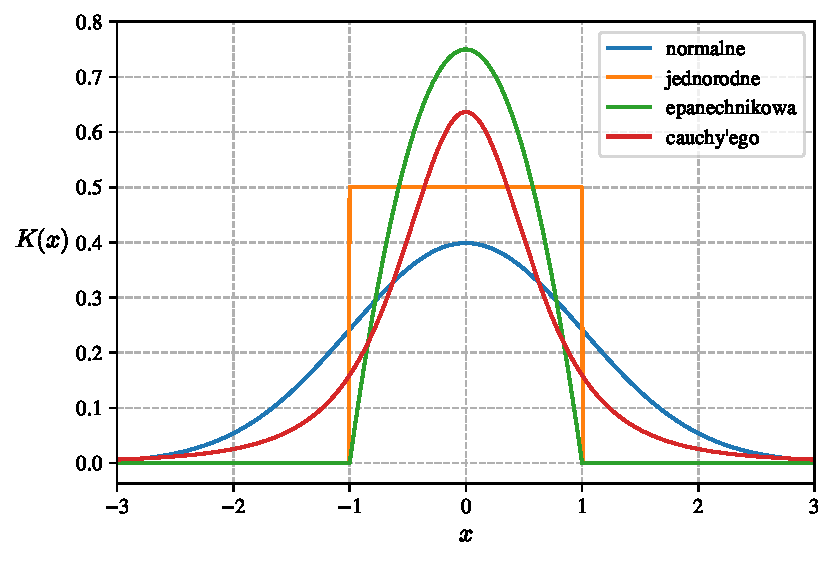
\includegraphics[scale=0.7]{kernels}
\caption{Wykresy wybranych jąder.}
\label{fig:kernels}
\end{figure}

\begin{exmp} \label{exmp:kde_construction}
Konstrukcja estymatora jądrowego dla $9$-elementowego zbioru jednowymarowych obserwacji o równych wagach, przedstawiona jest na rysunku \ref{fig:kde_construction}. Do konstrukcji wykorzystane zostało jądro normalne oraz arbitralnie ustalona wartość parametru wygładzania $h = 0.7$. Interpretacja wzoru \eqref{eq:kde2} jest następująca: dla pojedynczej obserwacji $x_i$ funkcja $K$ przesunięta o wektor $x_i$ i przeskalowana przez współczynnik $h$ reprezentuje oszacowanie rozkładu przy ustalonej wartości $x_i$. Dla $m$ niezależnych obserwacji $x_1, x_2, ..., x_m$ estymator gęstości prawdopodobieństwa przyjmuje formę sumy takich szacunków. Tak określona suma jest dodatkowo unormowana, aby zapewnić warunek $\int_\mathbb{R} \hat{f}(x) \mathrm{d}x = 1$.

\begin{figure}[H]
    \centering
    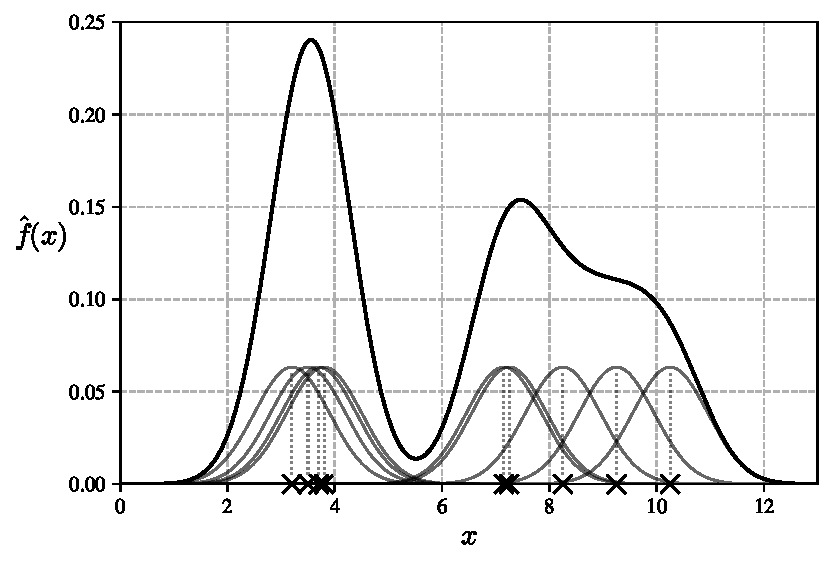
\includegraphics[scale=0.7]{kde_construction}
    \caption{Przykład konstrukcji estymatora jądrowego na zbiorze równoważnych obserwacji.}
    \label{fig:kde_construction}
\end{figure}
\end{exmp}

\begin{exmp}
Podobna konstrukcja estymatora jądrowego, zbudowanego na zbiorze obserwacji o różnych wagach, zaprezentowana została na rysunku \ref{fig:kde_construction_weighted}. Do konstrukcji estymatora wykorzystany został zbiór obserwacji z przykładu \ref{exmp:kde_construction}, jednak wzmocnione zostały dwie obserwacje najbardziej wysunięte na prawo (zwiększenie wag w stosunku $1:2:3$), z czego wynika zmieniony kształt otrzymanej krzywej gęstości $\hat{f}(x)$, w porównaniu do krzywej z przykładu \ref{exmp:kde_construction}.

\begin{figure}[H]
    \centering
    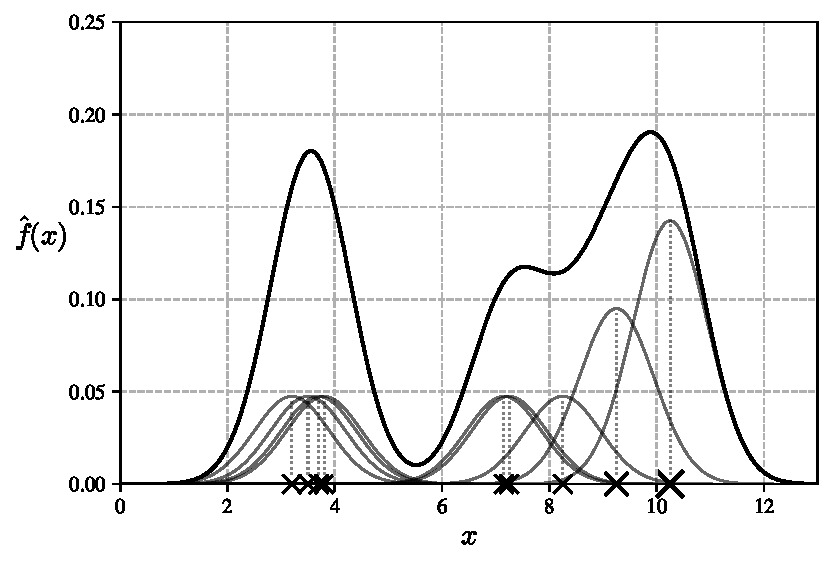
\includegraphics[scale=0.7]{kde_construction_weighted}
    \caption{Przykład konstrukcji estymatora jądrowego na zbiorze nierównoważnych obserwacji.}
    \label{fig:kde_construction_weighted}
\end{figure}
\end{exmp}

\section{Wyznaczanie parametru wygładzania} \label{sec:bandwidth_selection}

\textcolor{red}{(Opis i interpretacja) Kryterium scałkowanego błędu średniokwadratowego
\begin{equation} \label{eq:mise}
MISE = \int_{\mathbb{R}^n} \mathbb{E}[(\hat{f}(x) - f(x))^2] \mathrm{d}x
\end{equation}
Optymalizacja takiego kryterium względem $h$ daje (dla 1d)}
\begin{equation} \label{eq:opt_bandwidth1}
h_o = \left( \frac{R(K)}{U(K)^2 R(f^{\prime\prime}) m} \right)^\frac{1}{5},
\end{equation}
gdzie $U(g) = \int_{-\infty}^\infty x^2 g(x) \mathrm{d}x$ oraz $R(g) = \int_{-\infty}^\infty g(x)^2\mathrm{d}x$.

Bezpośrednie zastosowanie powyższych wzorów nie jest możliwe, gdyż nieznany jest rozkład $f$, a tym samym niemożliwe jest wyznaczenie $R(f^{\prime\prime})$. Wzory te jednak stanowią podstawę dla dogodnych metod suboptymalnych, takich jak:
\begin{enumerate}
\item metoda przybliżona \textcolor{red}{[referencja]}
\item metoda podstawień (\textcolor{red}{direct}) \textcolor{red}{[referencja]}
\item metoda podstawień (\textcolor{red}{solve-the-equation})
\item metoda \textcolor{red}{likelihood cross-validation}
\end{enumerate}
Powyższe metody stosowane są do zagadnień jednowymiarowych, a także do zagadnień wielowymiarowych, gdy używane jest jądro produktowe - wówczas obliczenia przeprowadza się wielokrotnie, odrębnie dla poszczególnych wspołrzędnych.

\subsection*{Metoda przybliżona}

Najłatwiejszym rozwiązaniem problemu nieznanego rozkładu $f$ jest arbitralne założenie, iż~$f$~jest rozkładem normalnym z odchyleniem standardowym oszacowanym na podstawie rozważanego zbioru obserwacji. Wówczas $R(f^{\prime\prime}) = \frac{3}{8 \sqrt{\pi} \hat{\sigma}^5}$, a wzór \eqref{eq:opt_bandwidth1} przyjmuje postać
\begin{equation} \label{eq:normal_reference}
\hat{h}_{pr} = \left( \frac{8 \pi^{1/2} R(K)}{3 U(K)^2 m} \right)^\frac{1}{5} \hat{\sigma},
\end{equation}
przy ważonym estymatorze odchylenia standardowego
\begin{equation}
\hat{\sigma} = \sqrt{\frac{m}{m-1} \sum_{i=1}^m w_i (x_i - \sum_{i=1}^m w_i x_i)^2}.
\end{equation}

\subsection*{Metoda podstawień (\textcolor{red}{direct})}

Metoda podstawień (\textcolor{red}{direct}) polega na idei "podstawienia" estymatora $\hat{\psi}_4$ nieznanej wielkości $R(f^{\prime\prime})$ we wzorze \eqref{eq:opt_bandwidth1}, wówczas wzór ten przyjmuje postać
\begin{equation} \label{eq:opt_bandwidth_modified}
\hat{h}_{po} = \left( \frac{R(K)}{U(K)^2 \hat{\psi}_4(g) m} \right)^\frac{1}{5},
\end{equation}
przy
\begin{equation} \label{eq:psi}
\hat{\psi}_r(g) = \frac{1}{m^2 g^{r+1}} \sum_{i=1}^m \sum_{j=1}^m \tilde K^{(r)} \left( \frac{x_i - x_j}{g} \right),
\end{equation}
gdzie $g$ jest parametrem wygładzania innym niż $h$, a jądro $\tilde K$ również może przyjmować inną postać niż $K$. W praktyce dogodnym wyborem $\tilde K$ jest jądro normalne, którego pożądaną cechą tutaj jest istnienie pochodnej dowolnego rzędu w całej dziedzinie. Symbol $^{(r)}$ oznacza pochodną funkcji rzędu $r$.

Łatwo zauważyć, że podstawienie wzoru \eqref{eq:psi} do wzoru \eqref{eq:opt_bandwidth_modified} nie jest wystarczające do wyliczenia $\hat{h}_{po}$, gdyż nieznany jest parametr $g$. W analogiczny sposób należy go wyznaczyć, podstawiając $\hat{\psi}_6$ za nieznaną wówczas wielkość $R(f^{(3)})$, napotykając na nieznany parametr $g_2$ na kolejnym poziomie zagnieżdzenia. W celu zatrzymania tak skonstruowanej nieskończonej pętli obliczeń, należy podstawić arbitralną wartość parametru wygładzania (np. wykorzystując wzór \eqref{eq:normal_reference} metody przybliżonej) na wybranym poziomie zagnieżdzenia. Stąd wynika pełna nazwa metody: metoda podstawień  (\textcolor{red}{direct}) $l$-tego poziomu.

Warto odnotować, iż przy $l=0$ metoda podstawień tożsama jest z metodą przybliżoną, a rozważania teoretyczne wskazują, aby wartość $l$ była równa conajmniej~$2$ (ze wskazaniem na $2$). Więcej na ten temat w \textcolor{red}{[referencje]}. \textcolor{red}{Złożoność kwadratowa.}

\begin{exmp}
Porównanie powyższych metod, zilustrowane zostało na rysunku \ref{fig:bandwidth_selection}. Po~lewej stronie rysunku przedstawione zostało porównanie metody przybliżonej z metodą podstawień rzędu 2, zastosowanych do konstrukcji estymatora jądrowego na jednowymiarowych danych wygenerowanych ze standardowego rozkładu normalnego $X \sim N(0,1)$, natomiast po prawej stronie rysunku zaprezentowane zostało podobne porównanie, uzupełnione o metodę podstawień rzędu 3, zastosowane na jednowymiarowych danych wygenerowanych z mieszaniny rozkładów normalnych \textcolor{red}{$X \sim 0.7 N(0,1) + 0.3 N(3,1)$}, reprezentującej rozkład dwumodalny. W obu zestawieniach wykorzystane zostało jądro normalne, a liczności zbiorów obserwacji równe są $m=100$. Przykład ten ilustruje przewagę metody przybliżonej nad metodą podstawień, gdy badany zbiór obserwacji pochodzi z rozkładu jednomodalnego. W przypadku rozkładów wielomodalnych, lepszej jakości estymację gęstości uzyskuje się przy wykorzystaniu metody podstawień.

\begin{figure}[H]
    \centering
    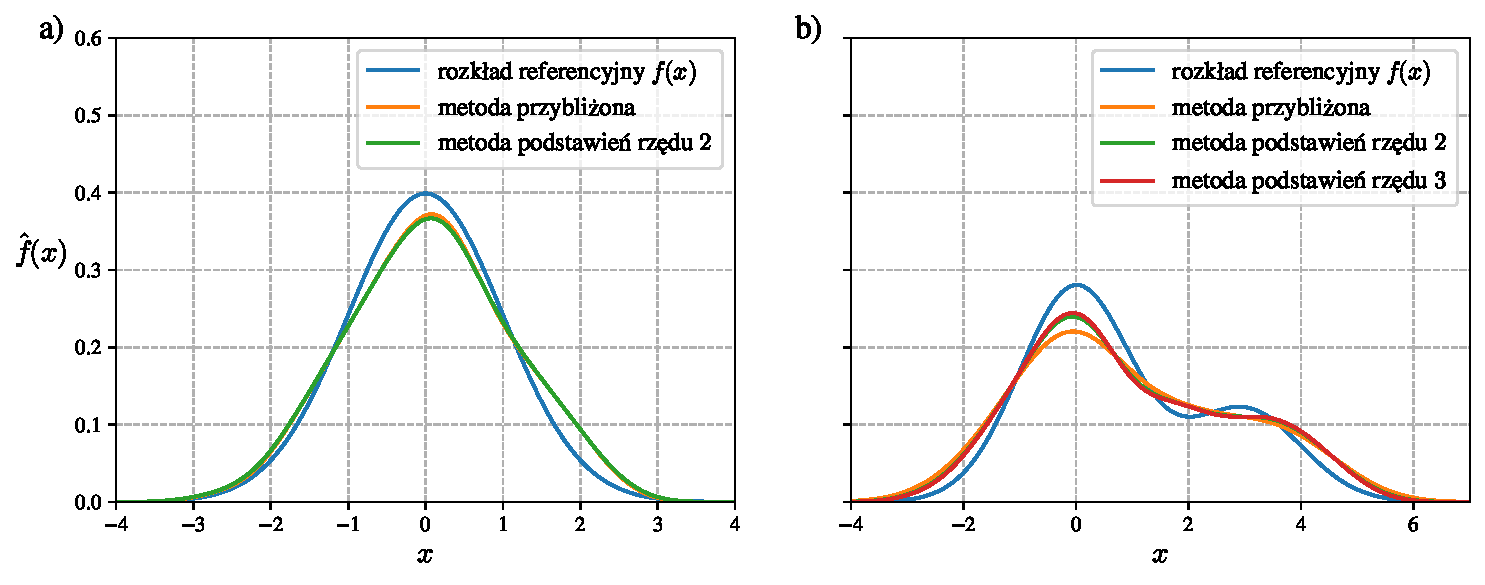
\includegraphics[scale=0.65]{bandwidth_selection}
    \caption{Porównanie metody przybliżonej do metody podstawień na przykładowych zbiorach obserwacji: jednomodalnym (lewa strona) oraz dwumodalnym (prawa strona).}
    \label{fig:bandwidth_selection}
\end{figure}
\end{exmp}

\subsection*{Metoda podstawień (solve-the-equation)}

\subsection*{Metoda likelihood cross-validation}

\section{Estymacja gęstości w ujęciu warunkowym} \label{sec:ckde}
Podstawowa koncepcja estymatora jądrowego \eqref{eq:kde1} zostanie teraz uogólniona do ujęcia warunkowego. Niech zatem podstawowe (objaśniające) atrybuty dane będą w postaci $n_X$-wymiarowej zmiennej $X$, natomiast atrybuty warunkowe reprezentowane będą przez $n_Y$-wymiarową zmienną $Y$. Ich kompozycja tworzy $(n_X+n_Y)$-wymiarową zmienną, której realizacje reprezentowne są przez $m$-elementowy zbiór obserwacji:
\begin{equation}\label{eq:ckde_dataset}
\begin{bmatrix}
x_1 \\
y_1
\end{bmatrix},
\begin{bmatrix}
x_2 \\
y_2
\end{bmatrix},
...,
\begin{bmatrix}
x_m \\
y_m
\end{bmatrix} \in \mathbb{R}^{n_X+n_Y},
\end{equation}
będący rozszerzeniem zbioru \eqref{eq:kde_dataset} o zmienną warunkową. Poszczególne elementy zbioru \eqref{eq:ckde_dataset} można interpretować jako wartości objaśniające $x_i$ przyjmowane w pomiarach, gdy wartości warunkowe przyjmują odpowiednie wartości $y_i$.

Przyjmując dodatkowo arbitralną wartość zmiennej warunkującej
\begin{equation}
y^* \in \mathbb{R}^{n_Y},
\end{equation}
estymator jądrowy warunkowego rozkładu zmiennej $X$ dla powyższej wartości warunkującej $y^*$ można zdefiniować przy pomocy funkcji $\hat{f}_{X \mid Y}(x \mid y^*):\mathbb{R}^{n_X} \rightarrow [0,\infty)$ określonej wzorem
\begin{equation} \label{eq:ckde}
\hat{f}_{X \mid Y}(x \mid y^*) = \frac{\hat{f}_{X,Y}(x,y^*)}{\hat{f}_Y(y)},
\end{equation}
gdzie $\hat{f}_{X,Y}$ jest bezwarunkowym estymatorem jądrowym łącznego rozkładu zmiennych $X$~oraz $Y$, natomiast $\hat{f}_Y$ jest bezwarunkowym estymatorem jądrowym zmiennej~$Y$, do~konstrukcji którego wykorzystuje się dodatnio określone jądro (np. jądro normalne), w celu zapewnienia warunku dodatniej wartości mianownika we wzorze \eqref{eq:ckde}. Gęstość warunkową, można zatem traktować jako gęstość "standardową" (bezwarunkową), której postać jest doprecyzowana przez wartość warunkującą $y^*$, adekwatną w badanym zagadnieniu.

W wyniku połączenia wzorów \eqref{eq:kde2} i \eqref{eq:ckde}, otrzymuje się warunkowy estymator jądrowy wyrażony wzorem
\begin{equation} \label{eq:ckde2}
\hat{f}_{X \mid Y}(x \mid y^*) = \frac{\sum_{i=1}^m w_i \prod_{j=1}^{n_X} \frac{1}{h_j} K \left( \frac{x_j-x_{i,j}}{h_j} \right) \prod_{j=1}^{n_Y} \frac{1}{h_{j+n_X}} K \left( \frac{y^*_j-y_{i,j}}{h_{j+n_X}} \right)}
{\sum_{i=1}^m w_i \prod_{j=1}^{n_Y} \frac{1}{h_{j+n_X}} K \left( \frac{y^*_j-y_{i,j}}{h_{j+n_X}} \right)}.
\end{equation}
Warto odnotować, iż uwagi dotyczące doboru jądra $K$ oraz wyznaczania parametru wygładzania $h \in \mathbb{R}^{n_X+n_Y}$, opisane odpowiednio w sekcji \ref{sec:kde} oraz \ref{sec:bandwidth_selection}, mają swoje zastosowanie również tutaj.
W dalszej części rozprawy, oznaczenie estymatora $\hat{f}_{X \mid Y}(x \mid y^*)$ zapisywane będzie w uproszczonej postaci $\hat{f}(x \mid y^*)$.

Wykorzystując następnie unormowany parametr
\begin{equation} \label{eq:d}
d_i = \frac{d_i^\prime}{\sum_{i=1}^m d_i^\prime},
\end{equation}
gdzie
\begin{equation} \label{eq:d_prim}
d_i^\prime = w_i \prod_{j=1}^{n_Y} K \left( \frac{y^*_j-y_{i,j}}{h_{j+n_X}} \right),
\end{equation}
można skonstruować uproszczone wyrażenie warunkowego estymatora jądrowego
\begin{equation} \label{eq:ckde3}
\hat{f}(x \mid y^*) = \sum_{i=1}^m d_i \prod_{j=1}^{n_X} \frac{1}{h_j} K \left( \frac{x_j-x_{i,j}}{h_j} \right).
\end{equation}
Każda wartość parametru $d_i$ charakteryzuje "odległość" wartości warunkującej $y^*$ od~wartości $y_i$, czyli tej wartości wektora warunkowego, dla którego uzyskano $i$-ty element zbioru \eqref{eq:ckde_dataset}. Owa "odległość" jest swego rodzaju uzupełnieniem wag $w_i$ poszczególnych obserwacji badanego zbioru, co uwidocznione jest w wizualnym podobieństwie wzoru warunkowego estymatora \eqref{eq:ckde3} oraz wzoru bezwarunkowego estymatora \eqref{eq:kde2}.

\begin{exmp}
Konstrukcja warunkowego estymatora jądrowego dla zbioru równoważnych obserwacji (przy parametrach $m=50, n_X=1, n_Y=1, y^*=1$) przedstawiona jest na rysunku \ref{fig:ckde_construction}. Do konstrukcji wykorzystane zostało jądro normalne oraz metoda przybliżona \eqref{eq:normal_reference} jako metoda wyznaczania parametru wygładzania. \textcolor{red}{(Interpretacja?) (z jakiego rozkładu losowano dane?)}

\begin{figure}[H]
    \centering
    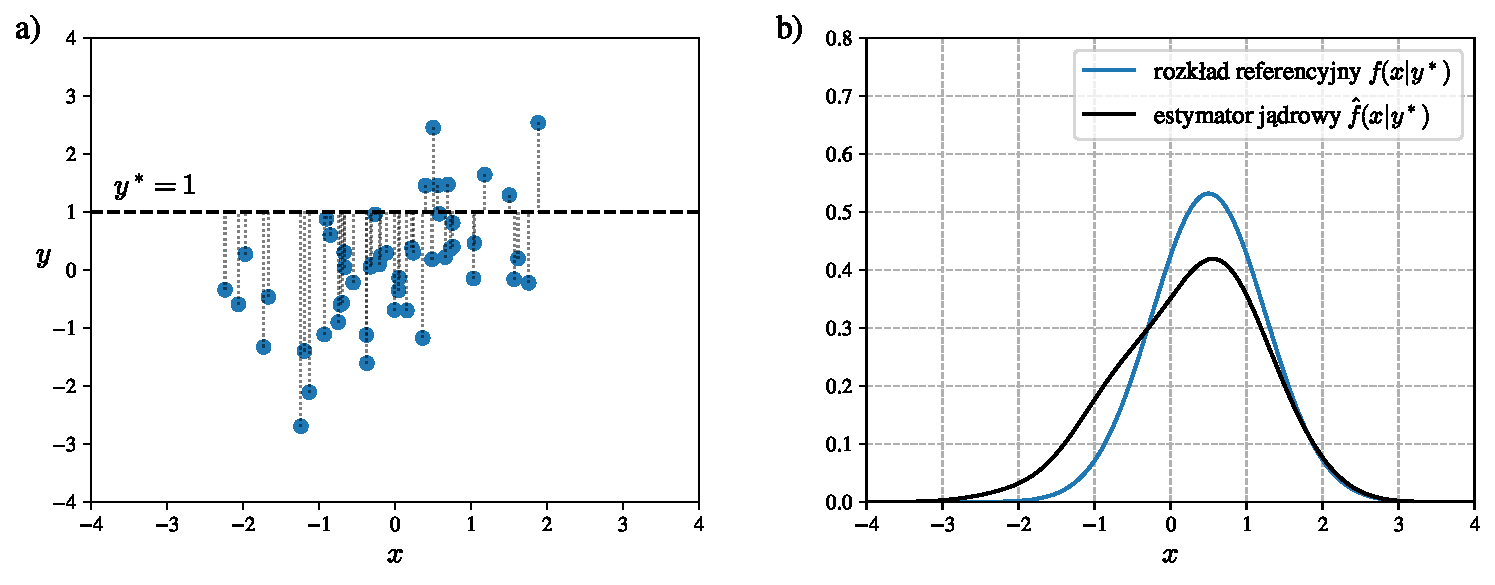
\includegraphics[scale=0.6]{ckde_construction}
    \caption{Przykład konstrukcji warunkowego estymatora jądrowego przy $y^*=1$.}
    \label{fig:ckde_construction}
\end{figure}
\end{exmp}

\chapter{Wykrywanie elementów nietypowych}

\textcolor{red}{Wstęp.}

\section{Procedura}

Dla $m$-elementowego zbioru obserwacji $x_i, y_i$ ($x_i \in \mathbb{R}^{n_X}, y_i \in \mathbb{R}^{n_Y}, i=1,2,...,m$) oraz ustalonego warunku $y^*$ buduje się warunkowy estymator za pomocą wzoru \eqref{eq:ckde3}. Procedura wykrywania elementów odstających:
\begin{enumerate}
\item Wylicza się zbiór: $\hat{f}(x_1 \mid y^*),\hat{f}(x_2 \mid y^*),...,\hat{f}(x_m \mid y^*)$
\item Zbiór ten sortujemy i zapisujemy jako $v_1,v_2,...,v_m$, tak, że $v_1 \leq v_2 \leq ... \leq v_m$
\item Dla takiego zbioru wylicza się estymator kwantyla rzędu $r$ oznaczony jako $\hat{q}_r$. Wartość $\hat{q}_r$ stanowi próg oddzielający wartości nietypowe od typowych
\begin{equation}
\hat{q}_r =
  \begin{cases}
    v_1 & \text{dla } r < d_1 \\
    \frac{\left( \sum_{i=1}^{k+1} d_i \right) - r}{d_{k+1}} v_k + \frac{r - \left( \sum_{i=1}^k d_i \right)}{d_{k+1}} v_{k+1} & \text{dla } r \geq d_1
  \end{cases}       
\end{equation}
parametr $k$ wyznacza się, tak aby spełniał warunek $\sum_{i=1}^k d_i \leq r < \sum_{i=1}^{k+1} d_i$. Parametr $d_i$ zdefiniowany jest wzorem \eqref{eq:d}.
\item Element nietypowy $x$ to taki, dla którego $\hat{f}(x | y^*) \leq q_r$, natomiast elementy typowy, to taki, dla którego $\hat{f}(x | y^*) > q_r$.
\end{enumerate}
Pozostaje parametr $r$ do wyznaczenia. Proponowaną domyślną wartością tego parametru jest $r=0.1$.
\begin{exmp}
\textcolor{red}{Opis przykładu}
\begin{figure}[H]
    \centering
    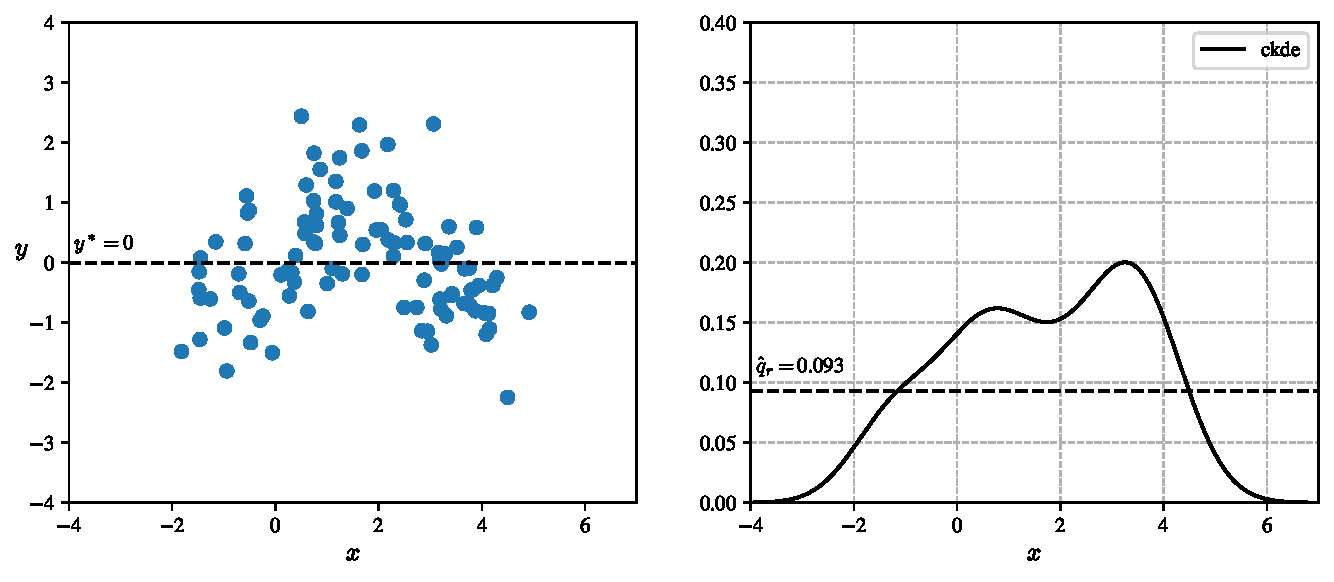
\includegraphics[scale=0.6]{ckde_outliers_detector_construction}
    \caption{\textcolor{red}{Podpis.}}
    \label{fig:ckde_outliers_detector_construction}
\end{figure}
\end{exmp}

\section{Wskaźnik jakości}

\section{Dopasowanie estymatora do wskaźnika jakości}

\section{Wyniki w postaci rozmytej i intuicjonistycznej}

\section{Wybrane metody alternatywne}

\chapter{Klasteryzacja}

\section{Procedura}

\section{Wskaźnik jakości}

\section{Dopasowanie estymatora do wskaźnika jakości}

\section{Wyniki w postaci rozmytej i intuicjonistycznej}

\section{Wybrane metody alternatywne}

\chapter{Klasyfikacja}

\textcolor{red}{Wstęp}

\section{Procedura}

Definiuje się zbiory danych (analogicznie do \eqref{eq:ckde_dataset}) dla $k$ klas:
\begin{equation}\label{eq:classification_dataset1}
\text{klasa 1:}
\begin{bmatrix}
x_1^1 \\
y_1^1
\end{bmatrix},
\begin{bmatrix}
x_2^1 \\
y_2^1
\end{bmatrix},
...,
\begin{bmatrix}
x_{m_1}^1 \\
y_{m_1}^1
\end{bmatrix} \in \mathbb{R}^{n_X+n_Y},
\end{equation}
\begin{equation}\label{eq:classification_dataset2}
\text{klasa 2:}
\begin{bmatrix}
x_1^2 \\
y_1^2
\end{bmatrix},
\begin{bmatrix}
x_2^2 \\
y_2^2
\end{bmatrix},
...,
\begin{bmatrix}
x_{m_2}^2 \\
y_{m_2}^2
\end{bmatrix} \in \mathbb{R}^{n_X+n_Y},
\end{equation}
\begin{equation}\label{eq:classification_datasetk}
\text{klasa $k$:}
\begin{bmatrix}
x_1^k \\
y_1^k
\end{bmatrix},
\begin{bmatrix}
x_2^k \\
y_2^k
\end{bmatrix},
...,
\begin{bmatrix}
x_{m_k}^k \\
y_{m_k}^k
\end{bmatrix} \in \mathbb{R}^{n_X+n_Y},
\end{equation}
o licznościach kolejno $m_1, m_2, ...,m_k$, dodatkowo $m=m_1+m_2+ ...+m_k$.

Dla tak przygotowanych danych, konstruuje się bayesowski klasyfikator, dzięki któremu będzie można sklasyfikować nową obserwację $x^\prime \in \mathbb{R}^{n_X}$, przy ustalonej wartości warunkującej $y^* \in \mathbb{R}^{n_Y}$, do jednej z $k$ klas.

Obserwacja $x^\prime$ należy do klasy $c$, określonej przez wyrażenie:
\begin{equation} \label{eq:bayes_classifier1}
\argmax_{c=1,2,...,k} P(c \mid x^\prime, y^*),
\end{equation}
gdzie $P(c \mid x^\prime, y^*)$ oznacza prawdopodobieństwo \textit{a posteriori} przynależności obserwacji $x^\prime$ do klasy $c$, przy ustalonej wartości warunkującej $y^*$. Z twierdzenia Bayesa:
\begin{equation} \label{eq:bayes_classifier2}
P(c \mid x^\prime, y^*) \propto \pi_c \hat{f}_c(x^\prime \mid y^*),
\end{equation}
gdzie $\pi_c$ oznacza prawdopodobieństwo \textit{a priori} przynależności obserwacji $x^\prime$ do klasy $c$, a $\hat{f}_c$ jest warunkowym estymatorem gęstości zbudowany na obserwacjach przynależących do klasy $c$. \textcolor{red}{(Aplikowanie $\pi_c$, założenie sumy równej 1 dla $P$)}

\begin{exmp}
\textcolor{red}{Opis przykładu}
\begin{figure}[H]
    \centering
    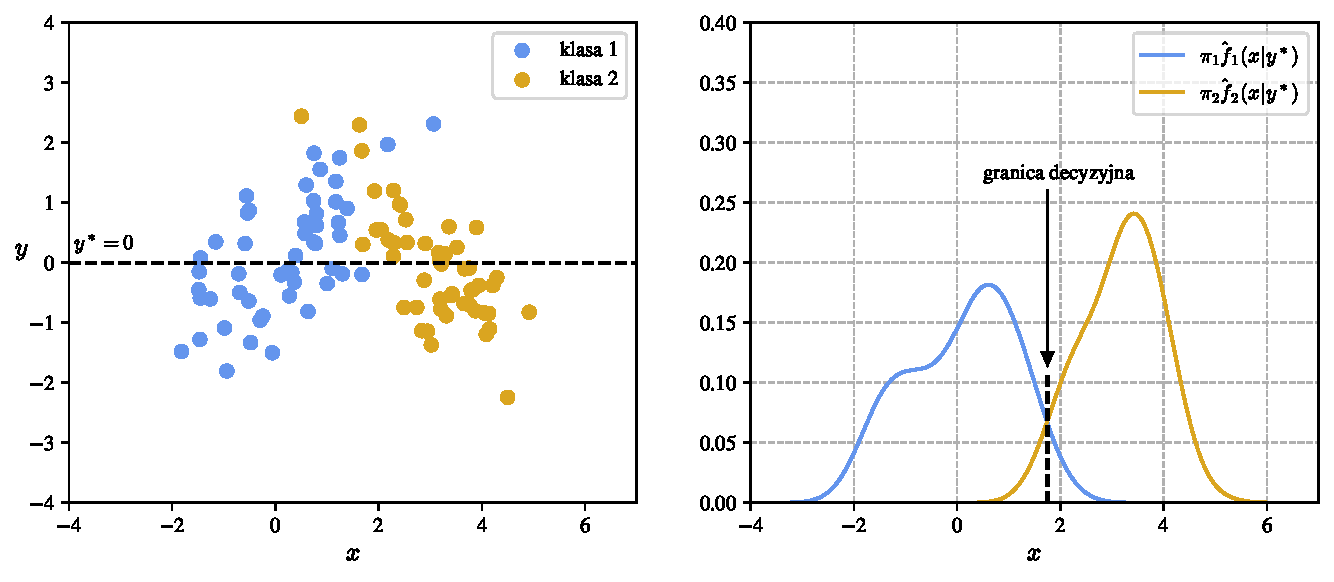
\includegraphics[scale=0.6]{ckde_classifier_construction}
    \caption{\textcolor{red}{Podpis.}}
    \label{fig:ckde_classifier_construction}
\end{figure}
\end{exmp}

\section{Wskaźnik jakości}
Klasyfikator ewaluowany jest przy pomocy wskaźnika jakości \textit{leave-one-out accuracy}.

Liczenie wskaźnika: wyciągamy $i$-tą obserwację $x_i$ ze zbioru danych użytego w procedurze i sprawdzamy czy ta obserwacja została dobrze sklasyfikowana, przy wartości warunkującej $y^*$. Powtarzamy to $m$-krotnie dla każdej obserwacji i uśredniamy wynik dobrze sklasyfikowanych obserwacji.

\textcolor{red}{Uwaga: musimy "ściągać" wartości $y_i$ do wartości $y^*$ i wtedy dopiero testować. Czym większy "dystans" $y_i$ do $y^*$ tym mniejszy sens ma taka klasyfikacja}

\textcolor{red}{Alternatywa 1: testujemy klasyfikator tylko na obserwacjach w określonym sąsiedztwie wartości warunkującej $y^*$}

\textcolor{red}{Alternatywa 2: testujemy klasyfikator na zupełnie nowym zbiorze testowym wygenerowanym z warunkowych rozkładów referencyjnych poszczególnych klas (prawdziwych rozkładów warunkowych $f_c(x \mid y^*)$). Dotyczy to syntetycznych zbiorów danych, gdy znamy postaci tych rozkładów.}

\section{Dopasowanie estymatora do wskaźnika jakości}

\section{Wyniki w postaci rozmytej i intuicjonistycznej}

\section{Wybrane metody alternatywne}

\chapter{Weryfikacja numeryczna}

\section{Dane syntetyczne}

\section{Dane rzeczywiste/realne}

\chapter{Podsumowanie}

\chapter{Notatki robocze}

\begin{enumerate}
\item Documentclass: report czy article?
\item Numeracja (i styl) stron
\item Marginesy stron
\end{enumerate}

\section{Matplotlib / Rysunki}

Ustawienia domyślne:
\begin{itemize}
	\item \textit{fontsize} 10 dla wszystkich elementów
	\item \textit{labelpad} 4
\end{itemize}
Moje wytyczne:
\begin{itemize}
	\item \textit{figsize} dla pojedynczego rysunku $(6, 4)$
	\item \textit{fontsize} 12 przy podpisach osi $x$ i $y$
	\item Zmienne w podpisach osi kursywą
	\item Elastyczny \textit{labelpad} dla osi $y$
	\item Tight\_layout(w\_pad=3/4)
\end{itemize}

% ==========  BIBLIOGRAFIA ==========
\newpage
\addcontentsline{toc}{chapter}{Bibliografia}
\bibliographystyle{abbrv}
\bibliography{bibliografia}


\end{document}